
\documentclass[aspectratio=169,10pt,english]{beamer}
\usepackage{beamer-hpicgs-min}

\usepackage{booktabs}
\usepackage{graphicx}
\usepackage{csquotes}
\usepackage{pdfpages}
\usepackage{gensymb}

\title{Mixed-Projection Treemaps}
\subtitle{A Novel Approach Mixing 2D and 2.5D Treemaps}
\titlegraphic{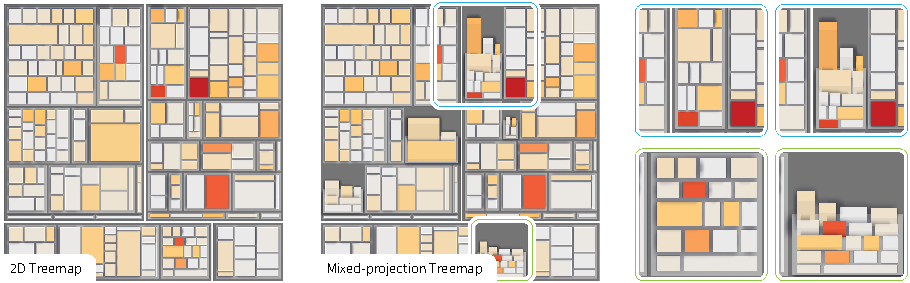
\includegraphics[width=0.96\textwidth]{images/teaser.pdf}}
\author{\underline{Daniel Limberger}, Willy Scheibel, Matthias Trapp, and Jürgen Döllner}
\institute{Hasso Plattner Institute, University of Potsdam, Germany}

\begin{document}

\setlength{\leftmargini}{10pt}

\begin{frame}[plain]
	\titlepage
\end{frame}

\begin{frame}[t]{Contributions of this Talk}

    \bigskip

    \Large\blueify{Introduction and Problem Statement}\medskip\normalsize

    An introduction to 2D and 2.5D treemaps and issues, e.g., depicting unknown data.

    \bigskip

    \Large\blueify{Node-Local Tilt}\medskip\normalsize

    A transformation that enables to dynamically mix different projections and seamless integration of 2.5D treemaps for region-of-interests into 2D treemaps.

    \bigskip

    \Large\blueify{Interactive Tilt Control}\medskip\normalsize

    An interaction concept that enables users to control the projection by means of manual and automated tilting, either providing explicit control or using animated state transitions, respectively.

\end{frame}

\begin{frame}[t]{Treemaps | Introduction}

    \bigskip

    \Large
    \blueify{Treemaps \cite{Johnson1991} are used to visualize tree-structured data,}

    \bigskip

    \begin{columns}

        \begin{column}{0.55\textwidth}
            \normalsize
            e.g., stock markets \cite{Wattenberg1999}, sensor data \cite{Mitchell2004}, business data \cite{Vliegen2006}, file systems \cite{Shneiderman1992}, software system information \cite{Wettel2008}

            \bigskip
            \begin{itemize}

                \pause
                \item[1.] non-spatial data is spatialized---it is given a gestalt that preserves the data's structure, e.g., rectangular treemaps use nested rectangles to depict nodes,

                \pause
                \item[2.] and data (attributes) are mapped to visual variables, i.e., properties of the rectangles (size and color).

            \end{itemize}

        \end{column}

        \begin{column}{0.38\textwidth}
            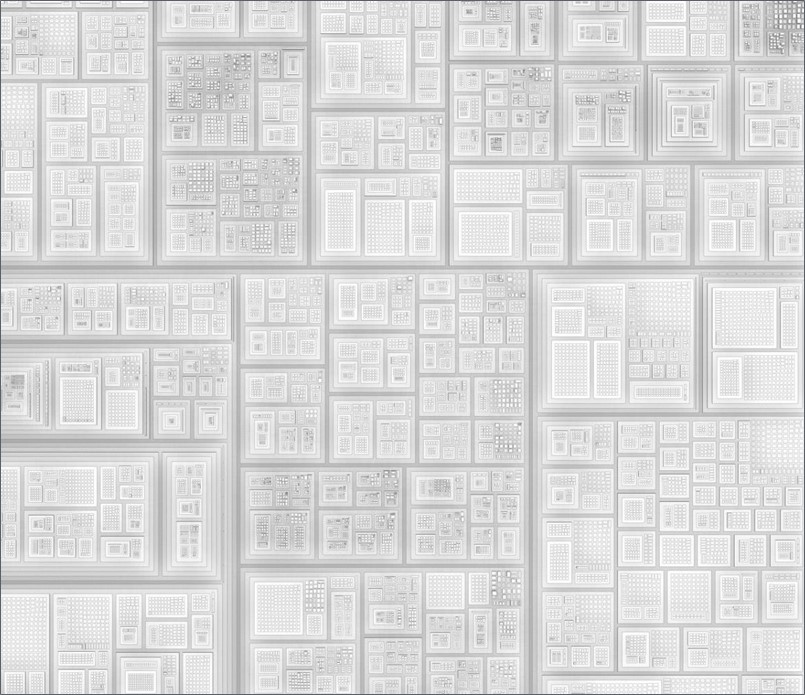
\includegraphics[width=1.8in]{images/flatmap.jpg}
        \end{column}

    \end{columns}

\end{frame}

\begin{frame}{Treemaps | Spatialization of Tree-structured Data}

    Leaf nodes are colored and have numerical weights, which can represent any associated attribute, e.g., file size.
    The weight of a parent node is defined by the sum of the weights of its child nodes.

    \begin{columns}[t]
        \begin{column}{0.47\textwidth}

            \centering
            \textcolor{CorporateBlue1}{Simple Graph}

        \end{column}

        \begin{column}{0.47\textwidth}

            \centering
            \textcolor{CorporateBlue1}{Rectangular Treemap}

        \end{column}

    \end{columns}

    \bigskip
    \centering
    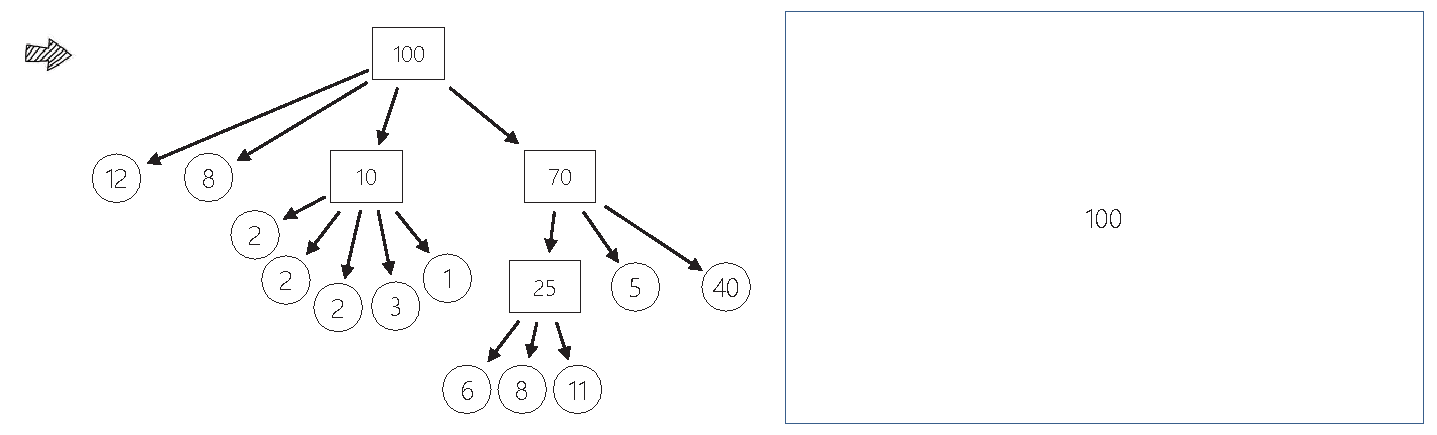
\includegraphics[height=0.475\paperheight]{images/treemap-create-1}

\end{frame}

\begin{frame}{Treemaps | Spatialization of Tree-structured Data}

    Leaf nodes are colored and have numerical weights, which can represent any associated attribute, e.g., file size.
    The weight of a parent node is defined by the sum of the weights of its child nodes.

    \begin{columns}[t]
        \begin{column}{0.47\textwidth}

            \centering
            \textcolor{CorporateBlue1}{Simple Graph}

        \end{column}

        \begin{column}{0.47\textwidth}

            \centering
            \textcolor{CorporateBlue1}{Rectangular Treemap}

        \end{column}

    \end{columns}

    \bigskip
    \centering
    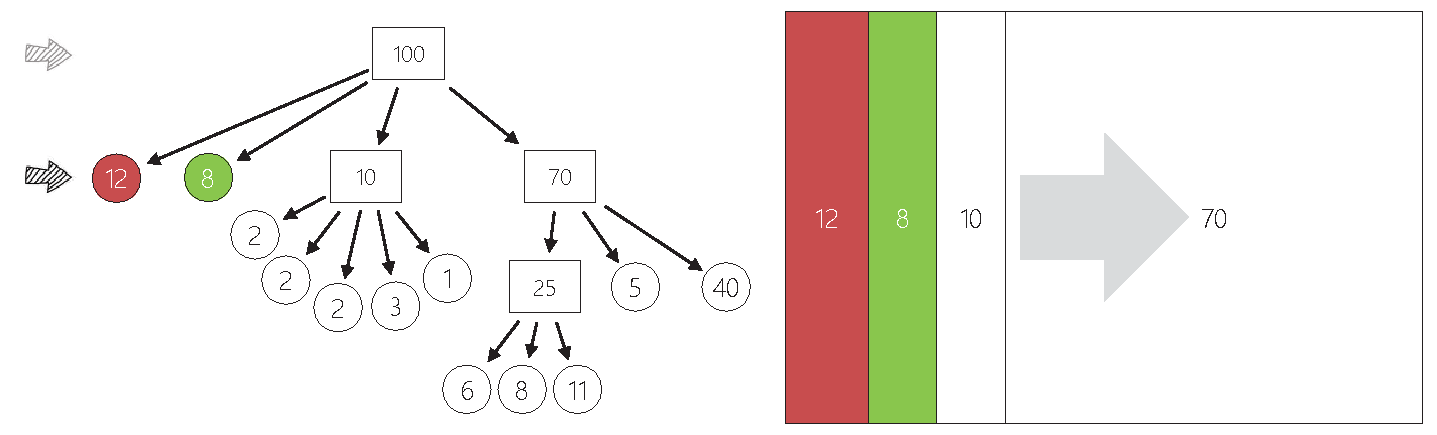
\includegraphics[height=0.475\paperheight]{images/treemap-create-2}

\end{frame}

\begin{frame}{Treemaps | Spatialization of Tree-structured Data}

    Leaf nodes are colored and have numerical weights, which can represent any associated attribute, e.g., file size.
    The weight of a parent node is defined by the sum of the weights of its child nodes.

    \begin{columns}[t]
        \begin{column}{0.47\textwidth}

            \centering
            \textcolor{CorporateBlue1}{Simple Graph}

        \end{column}

        \begin{column}{0.47\textwidth}

            \centering
            \textcolor{CorporateBlue1}{Rectangular Treemap}

        \end{column}

    \end{columns}

    \bigskip
    \centering
    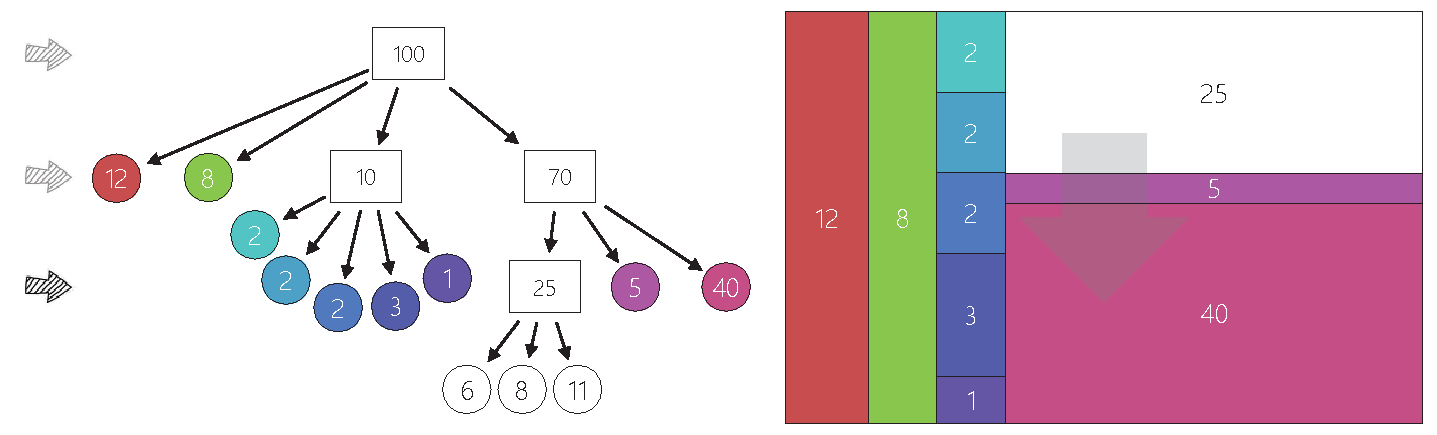
\includegraphics[height=0.475\paperheight]{images/treemap-create-3}

\end{frame}

\begin{frame}{Treemaps | Spatialization of Tree-structured Data}

    Leaf nodes are colored and have numerical weights, which can represent any associated attribute, e.g., file size.
    The weight of a parent node is defined by the sum of the weights of its child nodes.

    \begin{columns}[t]
        \begin{column}{0.47\textwidth}

            \centering
            \textcolor{CorporateBlue1}{Simple Graph}

        \end{column}

        \begin{column}{0.47\textwidth}

            \centering
            \textcolor{CorporateBlue1}{Rectangular Treemap}

        \end{column}

    \end{columns}

    \bigskip
    \centering
    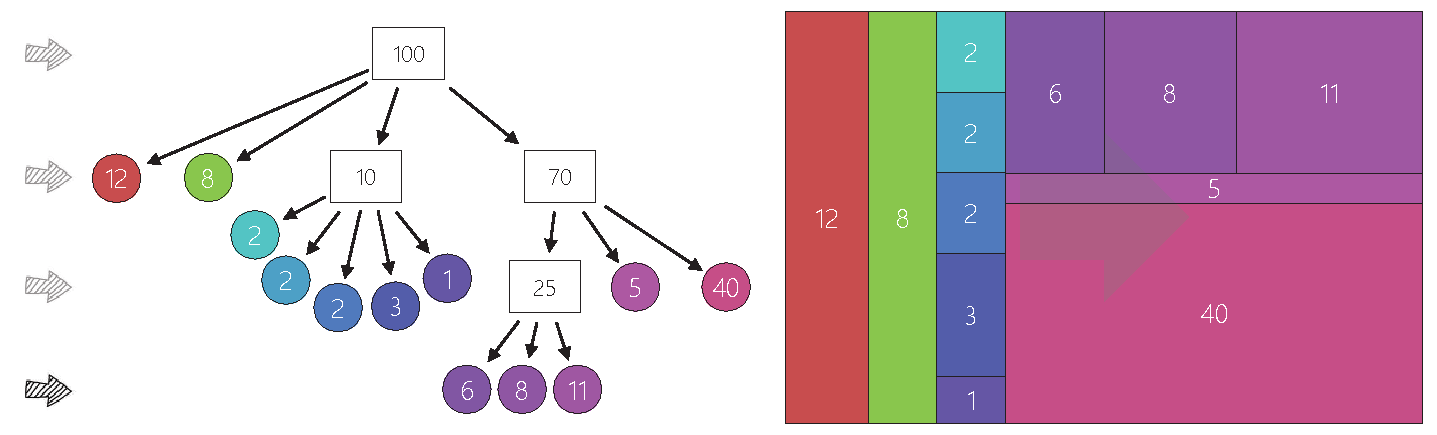
\includegraphics[height=0.475\paperheight]{images/treemap-create-4}

\end{frame}

\begin{frame}{Treemaps | Spatialization of Tree-structured Data}

    Leaf nodes are colored and have numerical weights, which can represent any associated attribute, e.g., file size.
    The weight of a parent node is defined by the sum of the weights of its child nodes.

    \begin{columns}[t]
        \begin{column}{0.47\textwidth}

            \centering
            \textcolor{CorporateBlue1}{Simple Graph}

        \end{column}

        \begin{column}{0.47\textwidth}

            \centering
            \textcolor{CorporateBlue1}{Rectangular Treemap}

        \end{column}

    \end{columns}

    \bigskip
    \centering
    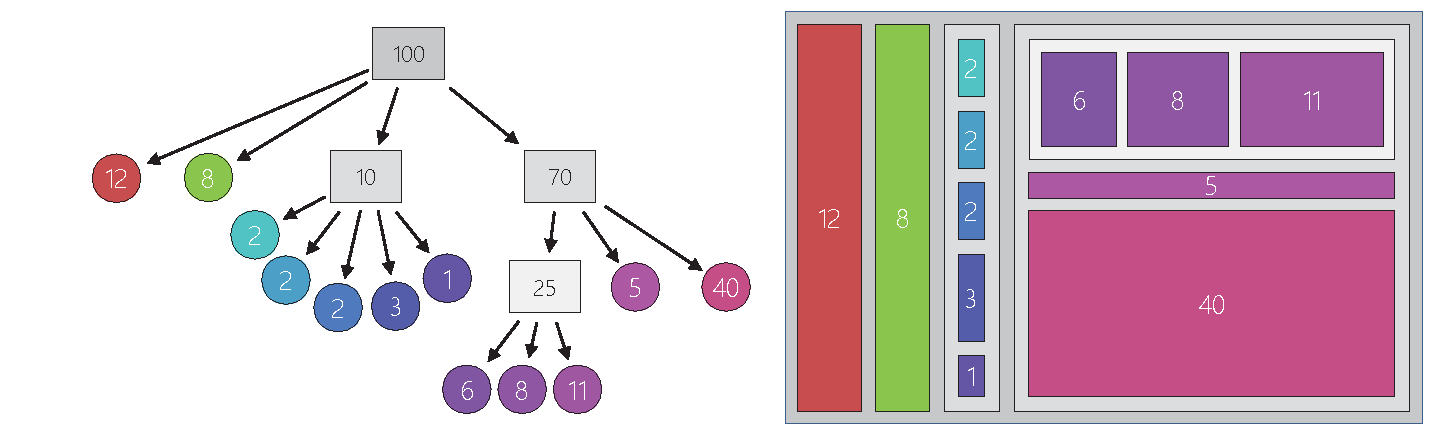
\includegraphics[height=0.475\paperheight]{images/treemap-create-5}

\end{frame}

{
\usebackgroundtemplate{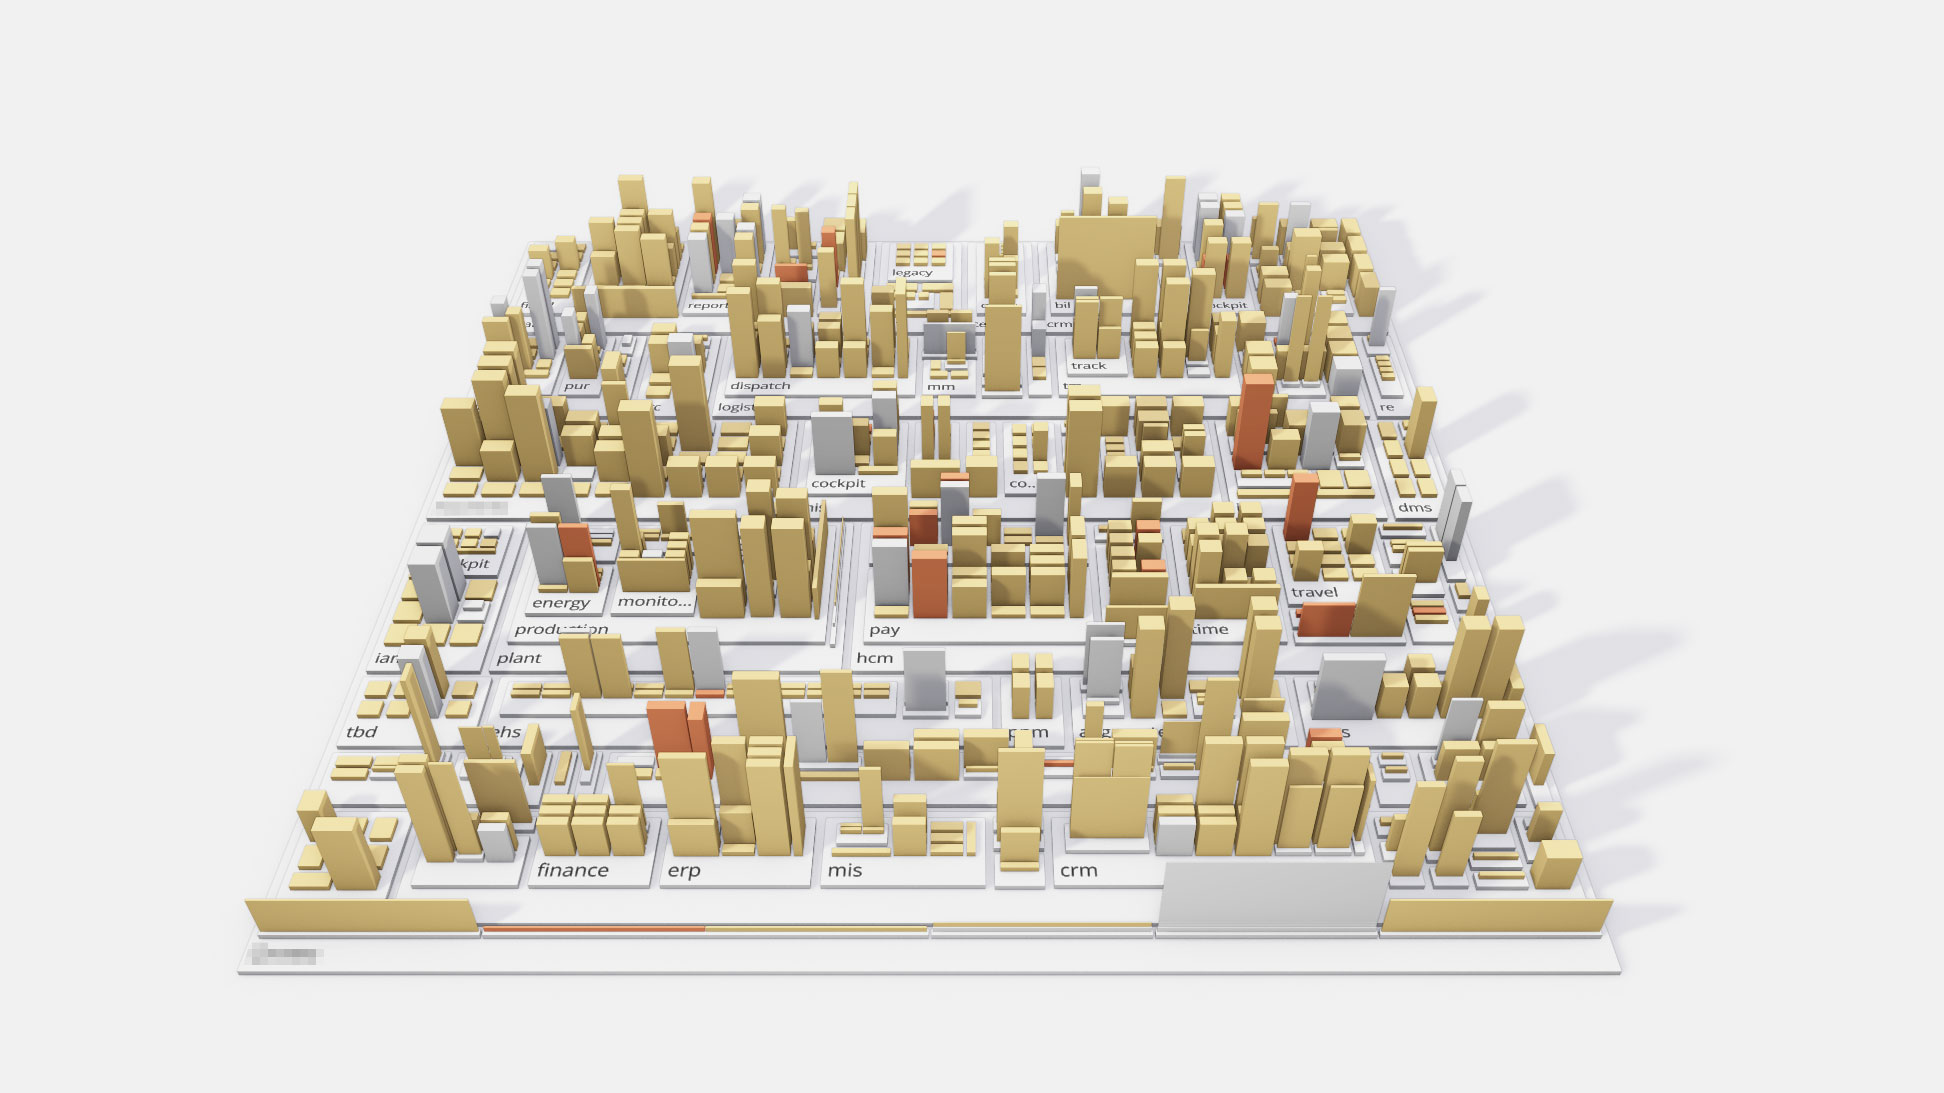
\includegraphics[height=\paperheight]{images/cemex-painter}}

\begin{frame}[t]{Treemaps | Adding Height as Visual Variable}

    \bigskip
    \bigskip
    2.5D Treemap \cite{Bladh2004}

\end{frame}
}

{
\usebackgroundtemplate{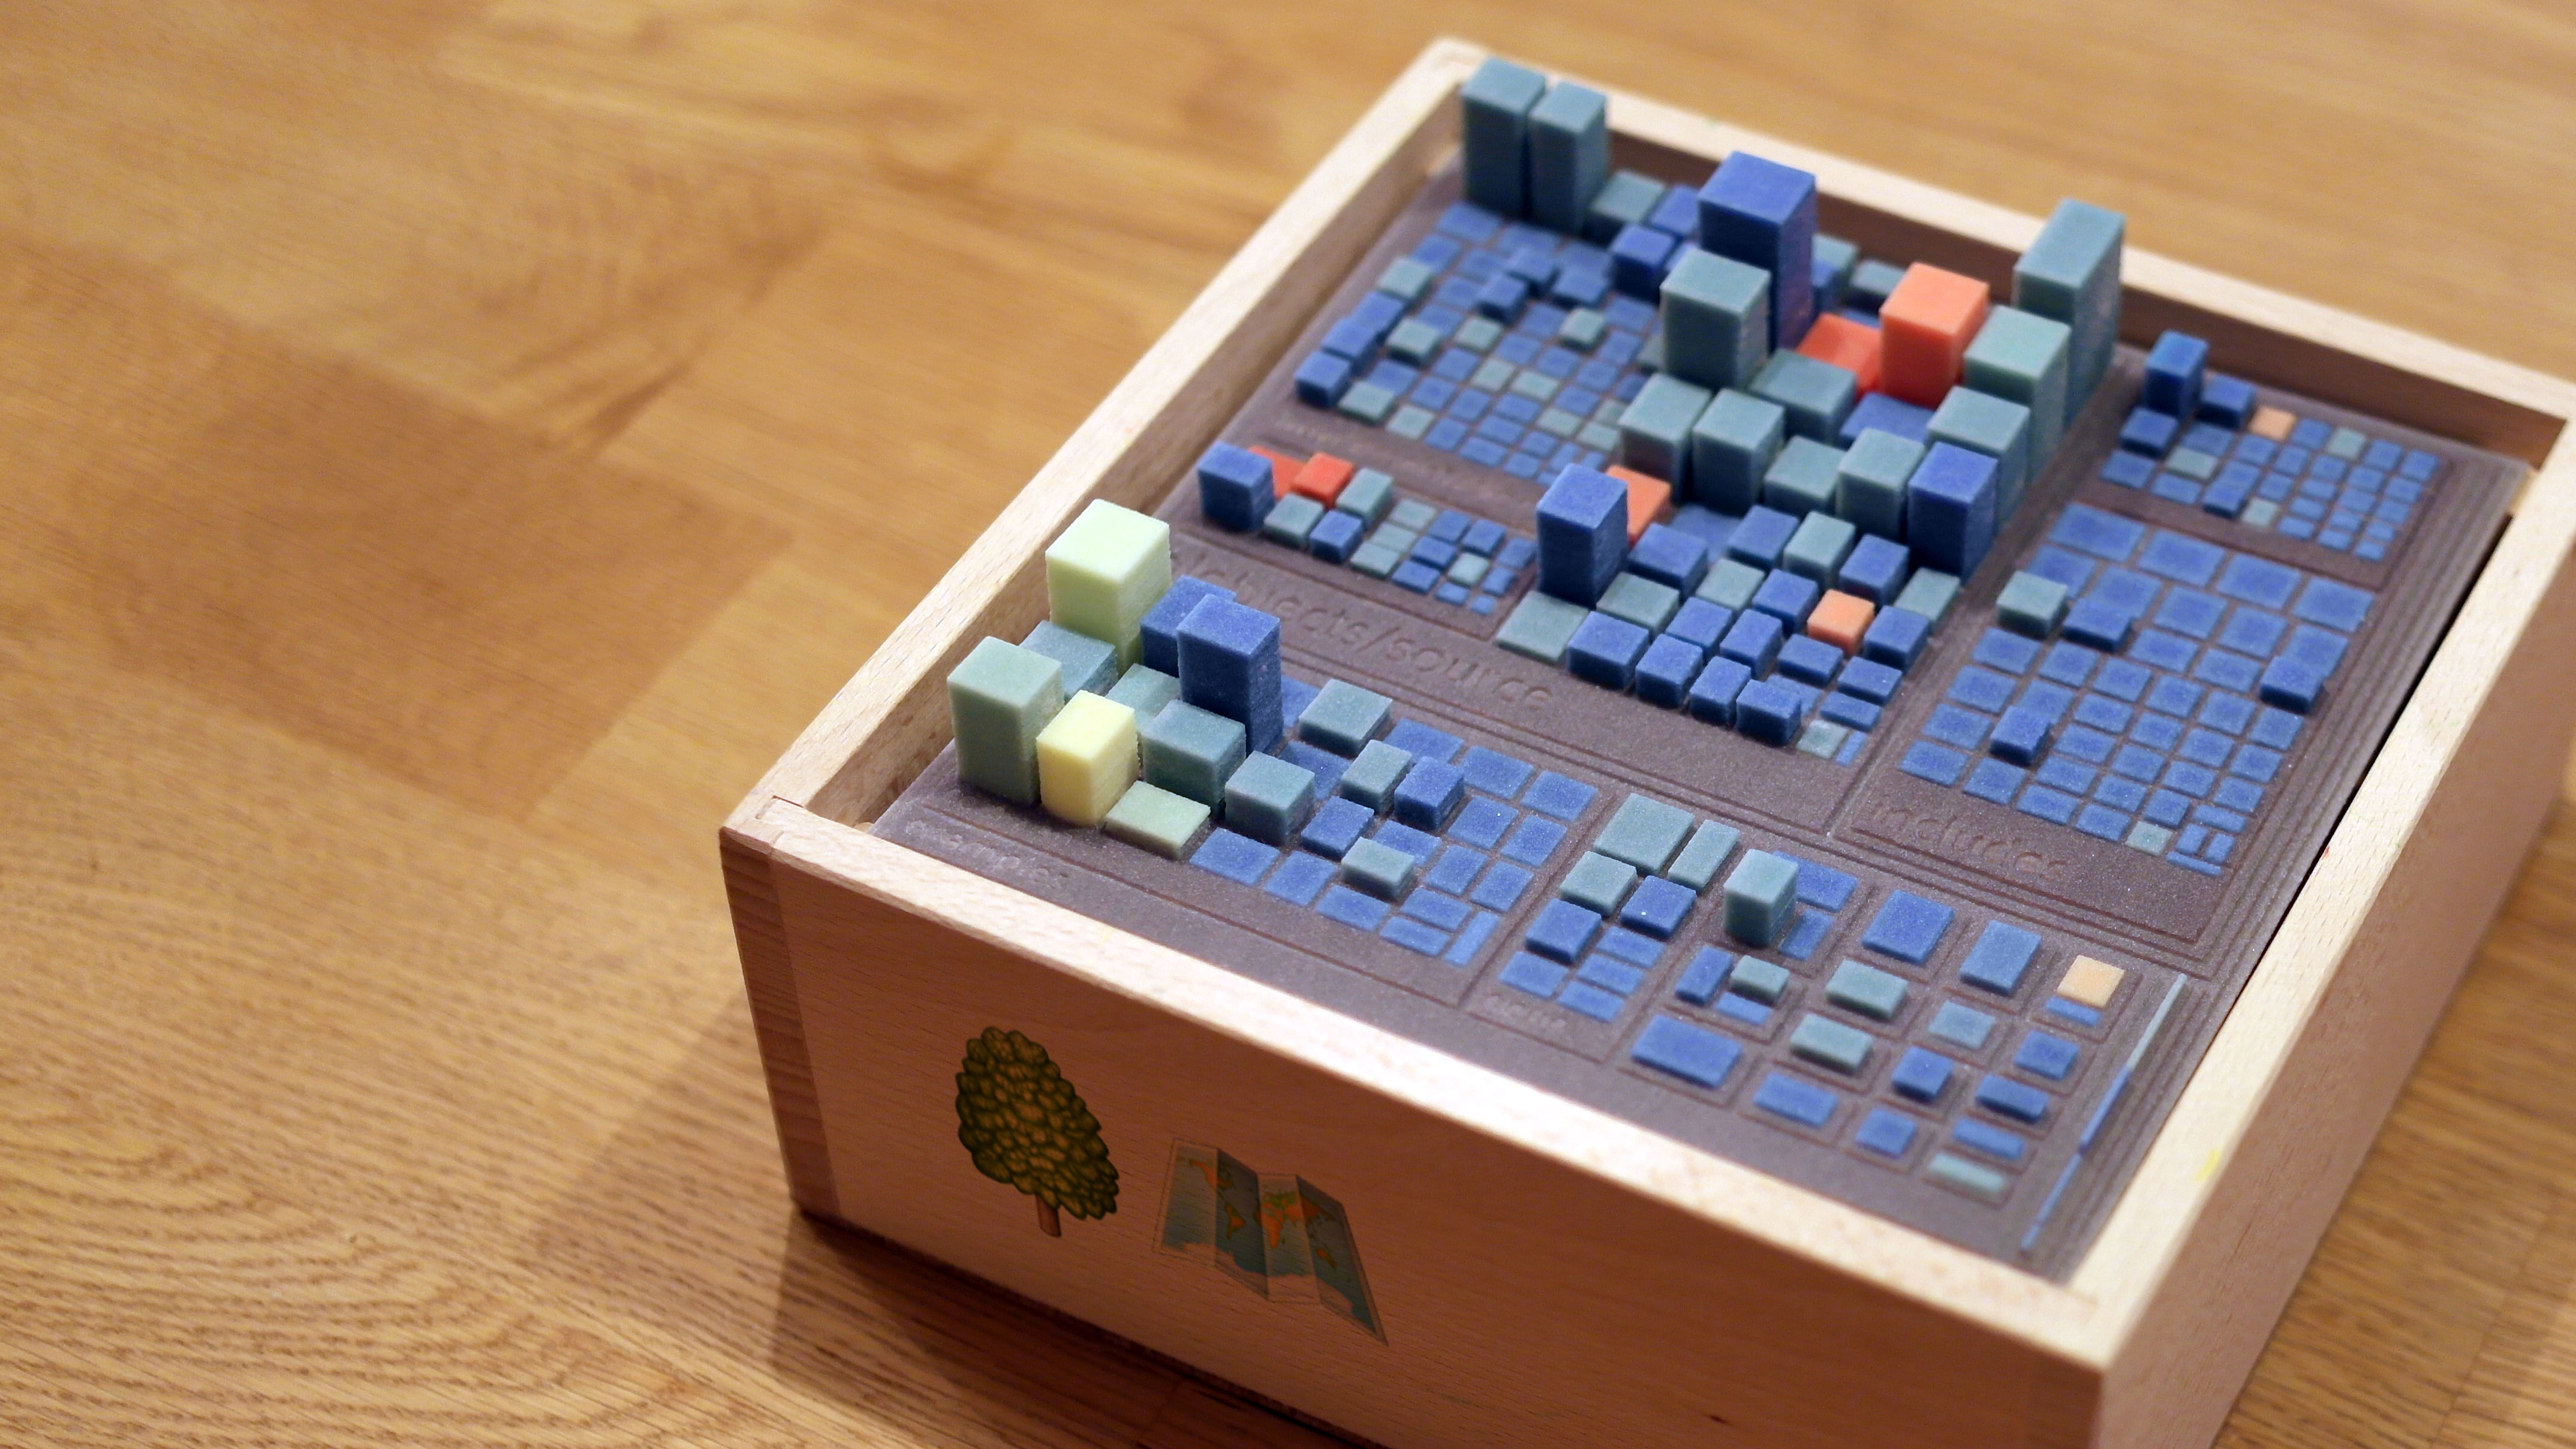
\includegraphics[height=\paperheight]{images/softwaremap-real}}

\begin{frame}{Software Maps | Basic Example}

    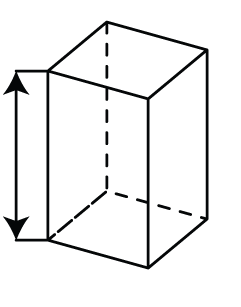
\includegraphics[width=0.35in]{images/visual-variables-height}

    \normalsize\textbf{\# complexity}

    \small nesting-level or McCabe

    \bigskip

    
\includegraphics[width=0.35in]{images/visual-variables-color}

    \normalsize\textbf{\# developers}

    \small that touched this unit

    \bigskip

    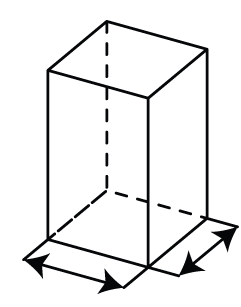
\includegraphics[width=0.35in]{images/visual-variables-footprint}

    \normalsize\textbf{\# lines-of-code}

\end{frame}
}

\begin{frame}[c]{Problem Statement | Exploration of Unknown Data}

    Exploration of unknown data is highly iterative and hinders use of \blueify{well-tuned map themes}.\\
    In order to reduce cognitive load, the following iterative approach is applied:

    \bigskip
    \bigskip
    {
        \scriptsize
        \begin{tabular}{cccc}

            \includegraphics[width=1.25in]<-1>{images/tierpark-placeholder}
            \includegraphics[width=1.25in]<2->{images/tierpark-weight} &
            \includegraphics[width=1.25in]<-2>{images/tierpark-placeholder}
            \includegraphics[width=1.25in]<3->{images/tierpark-color} &
            \includegraphics[width=1.25in]<-3>{images/tierpark-placeholder}
            \includegraphics[width=1.25in]<4>{images/tierpark-height}
            \includegraphics[width=1.25in]<5>{images/tierpark-placeholder}
            \includegraphics[width=1.25in]<6->{images/tierpark-mixed} &
            \includegraphics[width=1.25in]<-4>{images/tierpark-placeholder}
            \includegraphics[width=1.25in]<5>{images/tierpark-height}
            \includegraphics[width=1.25in]<6->{images/tierpark-height-disabled} \\

            \only<2->{\blueify{Topology, Weight}} &
            \only<3->{Topology, Weight, \blueify{Color}} &
            \only<4>{Topology, Weight, Color, \blueify{Height}}
            \only<6->{\blueify{Mixed-Projection}} &
            \only<5>{Topology, Weight, Color, \blueify{Height}}
            \only<6->{Full 2.5D (optional)}
        \end{tabular}
    }
    \bigskip

\end{frame}

\begin{frame}{Approach | Node-local Tilt}

    \LARGE
    \blueify{Tilt}
    \medskip

    \normalsize
    The rotation of an inner node (and its children) to enable exploration of additional attributes using visual variables common for 2.5D treemaps (e.g., height, transparency, sketchiness).
    \bigskip

    \pause
    \blueify{Any tilt comprises the following two node-local operations}:
    \begin{itemize}
        \item a tilt transformation $\Lambda = \left[T_C\right] T_A T^{-1}_R R T_R$
        \item and a tilt projection $\Gamma = \left(1 - t\right) P_0 + t P_1$.
    \end{itemize}
    \bigskip

\end{frame}

\begin{frame}[t]{Approach | Node-local Tilt | Transformation}

    \footnotetext[1]{$-1$ at bottom and $+1$ at top, $0$ at center.\label{footnote:range}\bigskip}

    \bigskip

    \begin{columns}

        \begin{column}{0.644\textwidth}

            \begin{itemize}
                \Large
                \only<1>{\item [$\Lambda$] $= \left[T_C\right] T_A T^{-1}_R R T_R$}
                \only<2>{\item [$\Lambda$] $= \left[T_C\right] T_A T^{-1}_R R \blueify{T_R}$}
                \only<3>{\item [$\Lambda$] $= \left[T_C\right] T_A T^{-1}_R \blueify{R} T_R$}
                \only<4>{\item [$\Lambda$] $= \left[T_C\right] T_A \blueify{T^{-1}_R} R T_R$}
                \only<5>{\item [$\Lambda$] $= \left[T_C\right] \blueify{T_A} T^{-1}_R R T_R$}
                \only<6>{\item [$\Lambda$] $= \left[\blueify{T_C}\right] T_A T^{-1}_R R T_R$}
                \normalsize
                \bigskip
                \bigskip

                \pause
                \item[$T_R$] shifts the node's rotation axis using a relative offset $\tau\in\left[-1,+1\right]$\textsuperscript{\ref{footnote:range}}

                \pause
                \item [$R$] rotates the node by the tilt angle $\alpha$

                \pause
                \pause
                \item [$T_A$] anchors the node to a preferred relative location $\upsilon\in\left[-1,+1\right]$\textsuperscript{\ref{footnote:range}}

                \pause
                \item [$T_C$] reduces occlusion introduced when using a perspective projection (optional).
            \end{itemize}

            \bigskip

        \end{column}

        \begin{column}{0.9in}
            \vspace{0.051in}
            \includegraphics[width=\textwidth]<1>{images/transformations-1}
            \includegraphics[width=\textwidth]<2>{images/transformations-2}
            \includegraphics[width=\textwidth]<3>{images/transformations-3}
            \includegraphics[width=\textwidth]<4>{images/transformations-4}
            \includegraphics[width=\textwidth]<5>{images/transformations-5}
            \includegraphics[width=\textwidth]<6>{images/transformations-6}
        \end{column}

    \end{columns}

\end{frame}

\begin{frame}{Approach | Node-local Tilt | Transformation}

    \scriptsize
    Tilt transformation $\Lambda$ of an inner-node $n$ with perspective projection:

    \medskip
    {
    \centering

    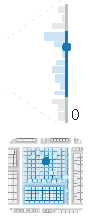
\includegraphics[width=0.9in]{images/transformations-1}
    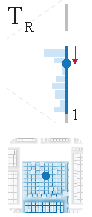
\includegraphics[width=0.9in]{images/transformations-2}
    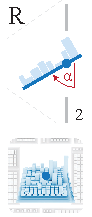
\includegraphics[width=0.9in]{images/transformations-3}
    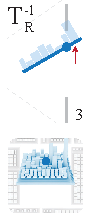
\includegraphics[width=0.9in]{images/transformations-4}
    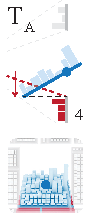
\includegraphics[width=0.9in]{images/transformations-5}
    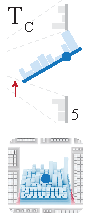
\includegraphics[width=0.9in]{images/transformations-6}
    }
    \medskip
    $n$ is (1) translated by $T_R$ for (2) rotation by $R$ with $\alpha=60\degree$ at the local tilt offset $\tau=0.5$. After (3) translating $n$ ($T^{-1}_R$) it is (4) moved to the bottom anchor by $T_A$ with $\upsilon=-1$ and, (5) shifted up again by $T_C$ in order to reduce the occlusion caused by the perspective projection.

\end{frame}

\begin{frame}[t]{Approach | Node-local Tilt | Projection}

    \bigskip

    \begin{columns}

        \begin{column}{0.66\textwidth}

            \begin{itemize}
                \Large
                \item[$\Gamma$] $= \left(1 - t\right) P_0 + t P_1$ \\

                \normalsize
                \bigskip
                \bigskip

                \item[] mixes any two given projections $P_0$ and $P_1$ with respect to the node local tilt angle $\alpha$ and a global angular threshold $\beta$ with

                \pause
                \item[$P_0$] as orthographic projection,

                \pause
                \item [$P_1$] as perspective projection that cover the exact same treemap region, and

                \pause
                \item [$t$] $= \alpha\beta^{-1}$, clamped to $\left[0,1\right]$.

            \end{itemize}

            \bigskip

        \end{column}

        \begin{column}{0.9in}

        \end{column}

    \end{columns}

\end{frame}

\begin{frame}{Approach | Node-local Tilt | Parametrization for $\alpha = 60\degree$}

    \footnotesize

    \begin{tabular}{lcccc}

        & Ortho &  Persp, $\tau=-1$ & Persp, $\tau=0$ & Persp, $\tau=+1$ \medskip\\

        $\upsilon=-1$ (bottom) &
        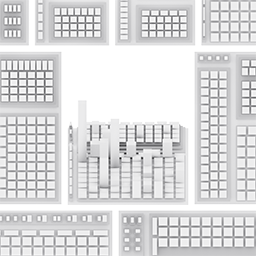
\includegraphics[width=0.7in]{images/matrix/60-b-b-ortho} &
        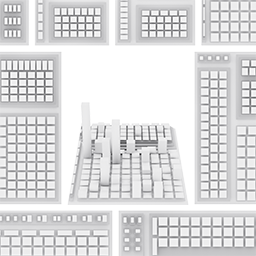
\includegraphics[width=0.7in]{images/matrix/60-b-b-persp} &
        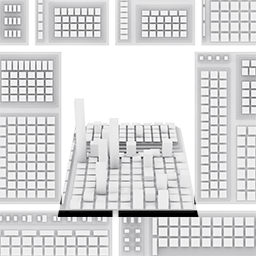
\includegraphics[width=0.7in]{images/matrix/60-b-c-persp} &
        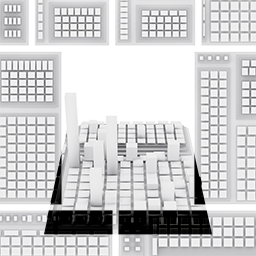
\includegraphics[width=0.7in]{images/matrix/60-b-f-persp} \medskip\\

        $\upsilon=0$ (center) &
        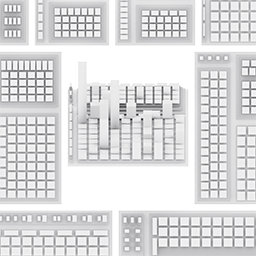
\includegraphics[width=0.7in]{images/matrix/60-c-b-ortho} &
        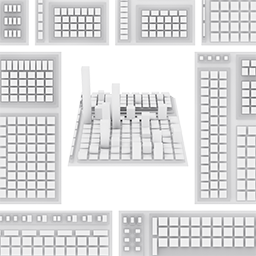
\includegraphics[width=0.7in]{images/matrix/60-c-b-persp} &
        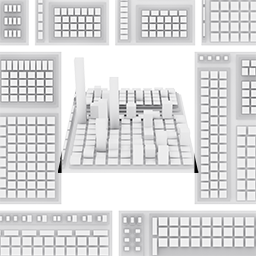
\includegraphics[width=0.7in]{images/matrix/60-c-c-persp} &
        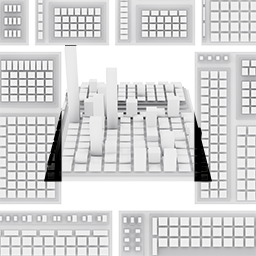
\includegraphics[width=0.7in]{images/matrix/60-c-f-persp} \medskip\\

        $\upsilon=+1$ (top) &
        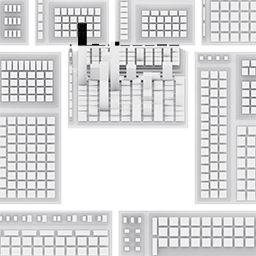
\includegraphics[width=0.7in]{images/matrix/60-t-b-ortho} &
        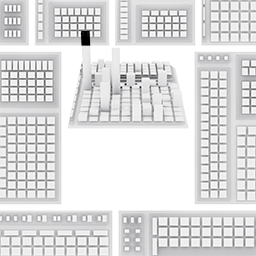
\includegraphics[width=0.7in]{images/matrix/60-t-b-persp} &
        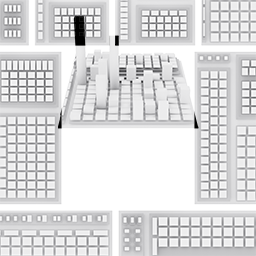
\includegraphics[width=0.7in]{images/matrix/60-t-c-persp} &
        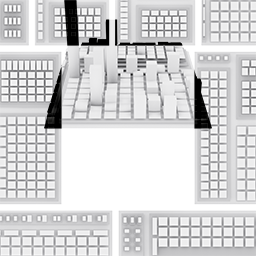
\includegraphics[width=0.7in]{images/matrix/60-t-f-persp}

    \end{tabular}

\end{frame}

\begin{frame}{Approach | Interactive Tilt Control}

    \LARGE
    \blueify{Interaction}
    \medskip

    \normalsize
    Users can interact directly with treemap nodes based on direct manipulation metaphors.
    \bigskip

    \pause
    \blueify{For it we suggest two similar tilt modes}:
    \begin{itemize}
        \item \blueify{automated tilt} enabling users to invoke a preset tilt angle or un-tilt any node by a single input event,\\e.g., click/touch to an inner node,

        \item \blueify{manual tilt} enabling users to increase and decrease the tilt angle of any node seamlessly,\\e.g., via click/touch to an inner node and vertical drag down.
    \end{itemize}
    \bigskip

\end{frame}

\begin{frame}{Approach | Automated Tilt (local)}

\end{frame}

\begin{frame}{Approach | Manual Tilt (global)}

\end{frame}

\begin{frame}[t]{Future Work}

    \bigskip

    \begin{columns}

        \begin{column}{0.3\textwidth}

        \centering
        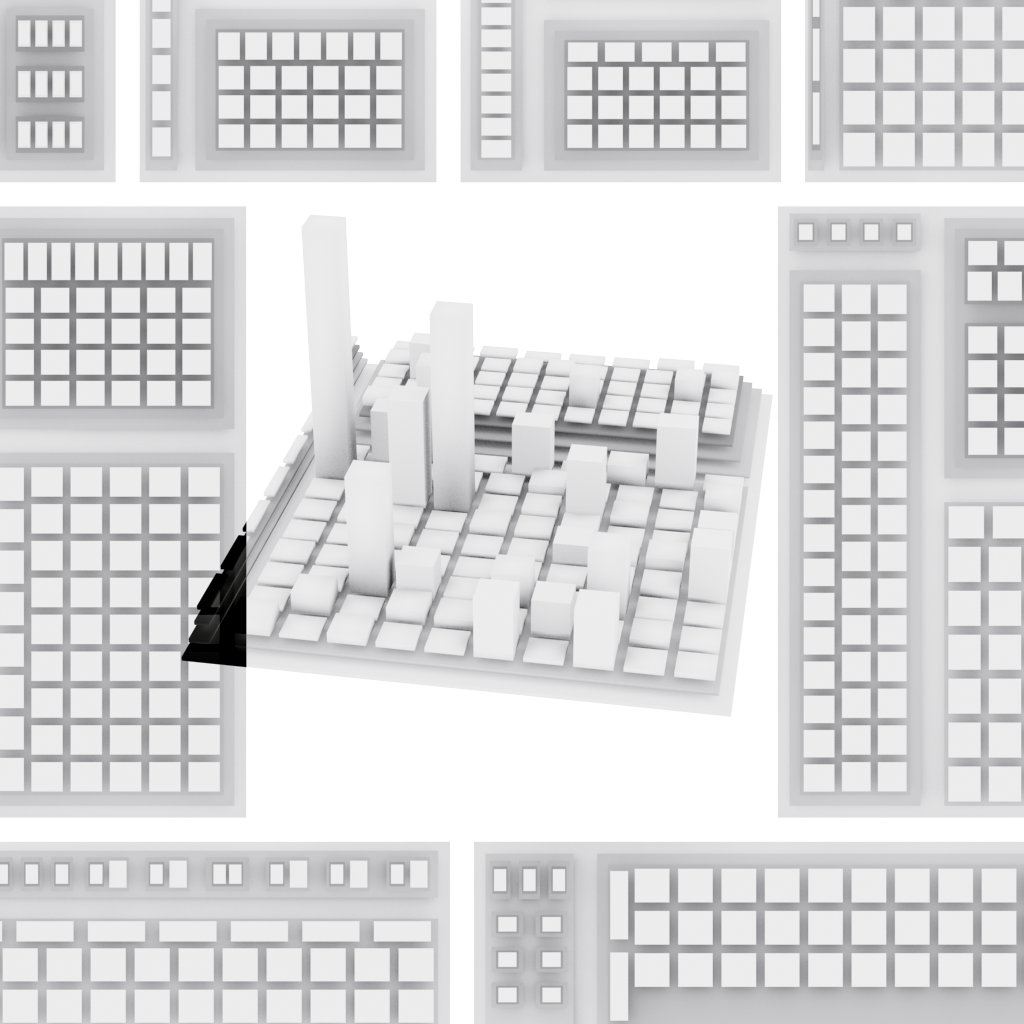
\includegraphics[height=1.1in]{images/occlusion-rotate-+15}\medskip\\
        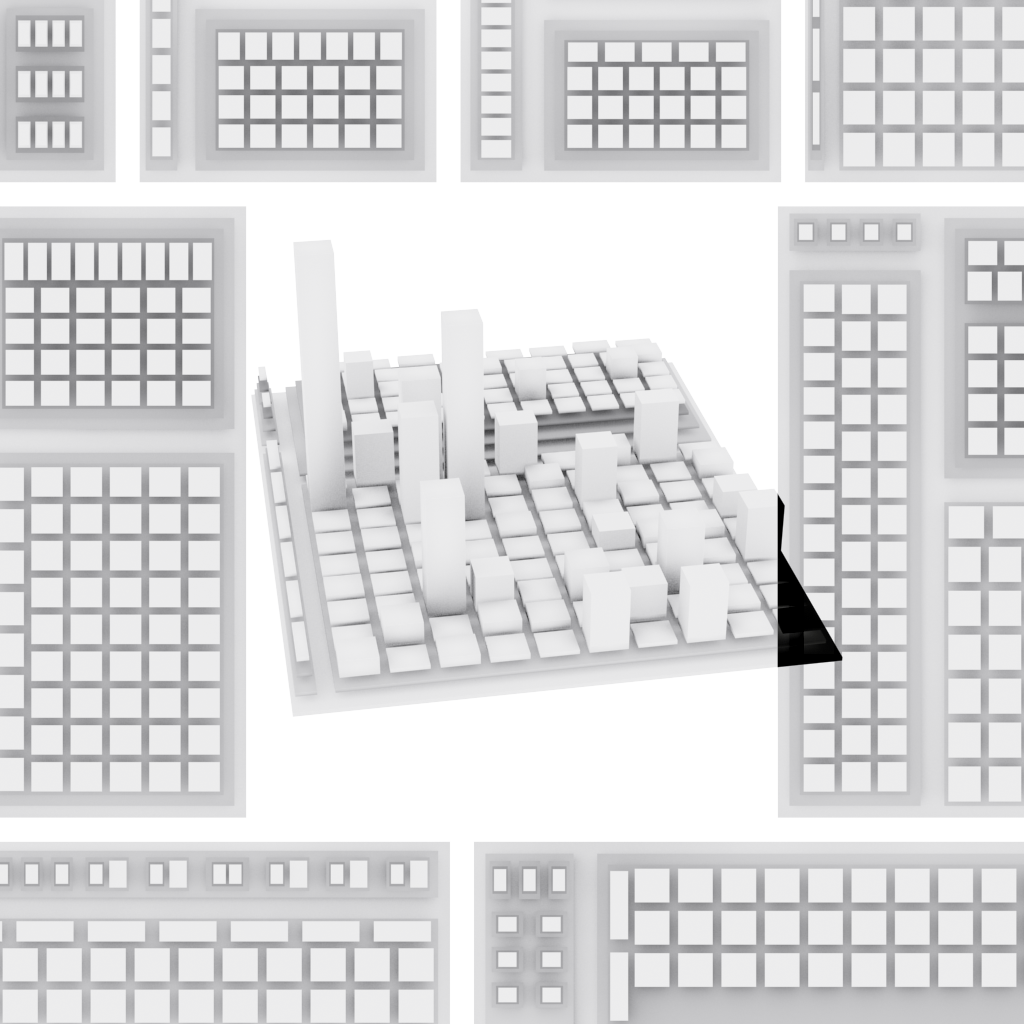
\includegraphics[height=1.1in]{images/occlusion-rotate--10}

        \smallskip
        Additional Rotation

        \end{column}

        \begin{column}{0.3\textwidth}

        \centering
        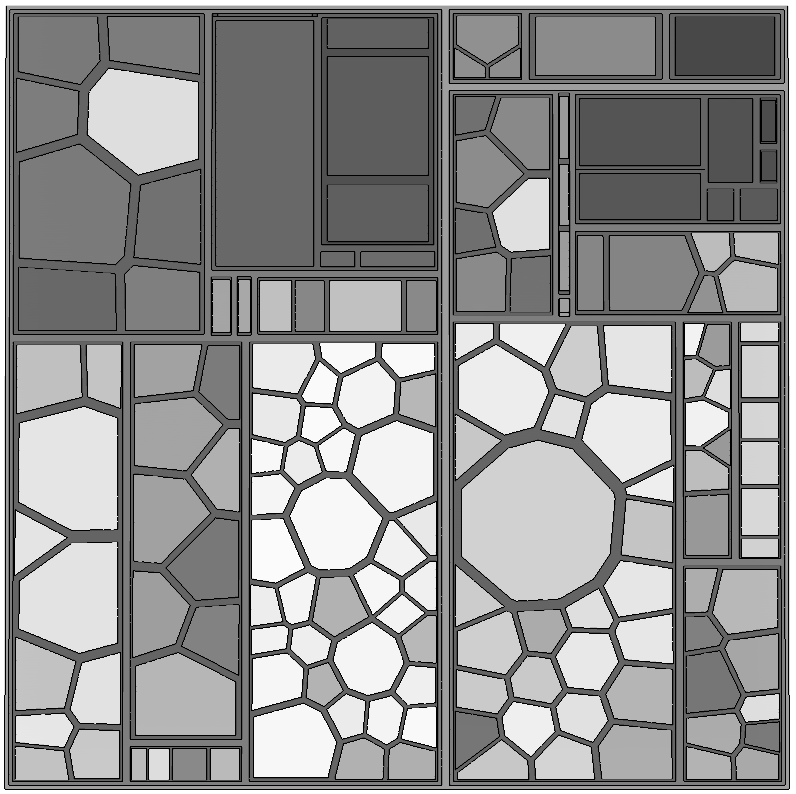
\includegraphics[height=1.1in]{images/future-mixed-layout}\medskip\\
        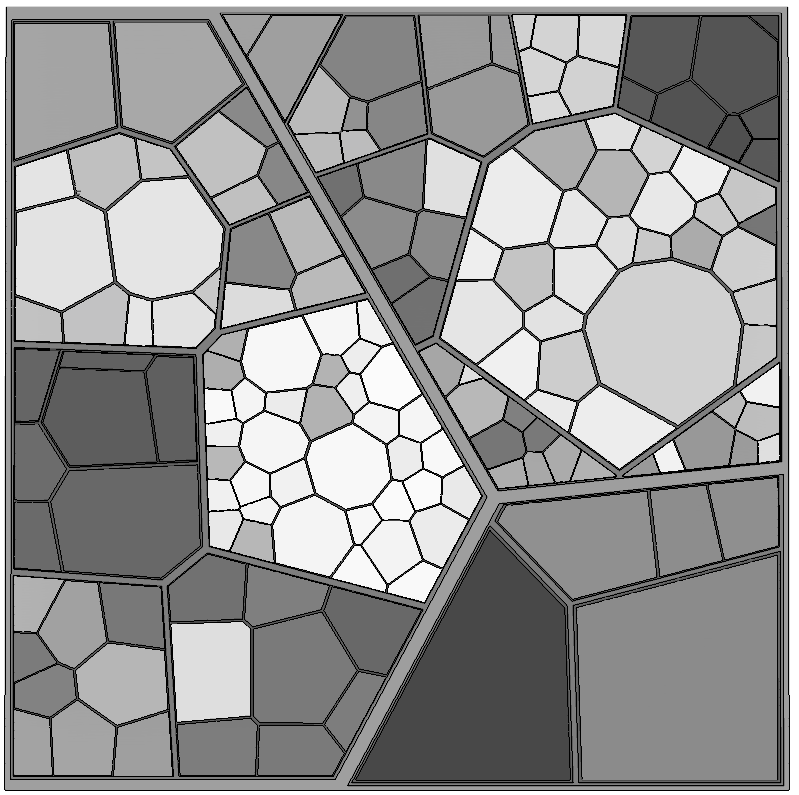
\includegraphics[height=1.1in]{images/future-voronoi}

        \smallskip
        Non-rectangular Treemaps \cite{Hahn2017}

        \end{column}

        \begin{column}{0.3\textwidth}

        \centering
        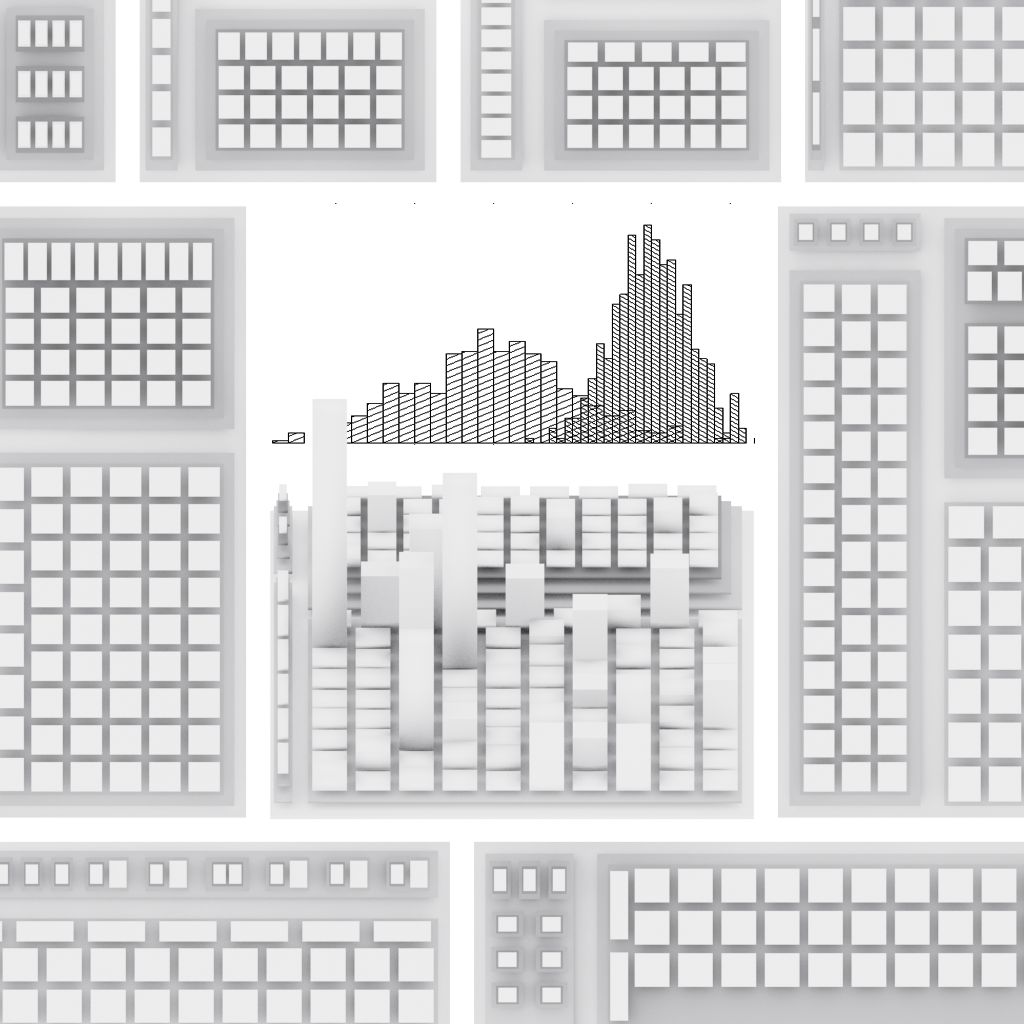
\includegraphics[height=1.1in]{images/future-ortho-histo}\medskip\\
        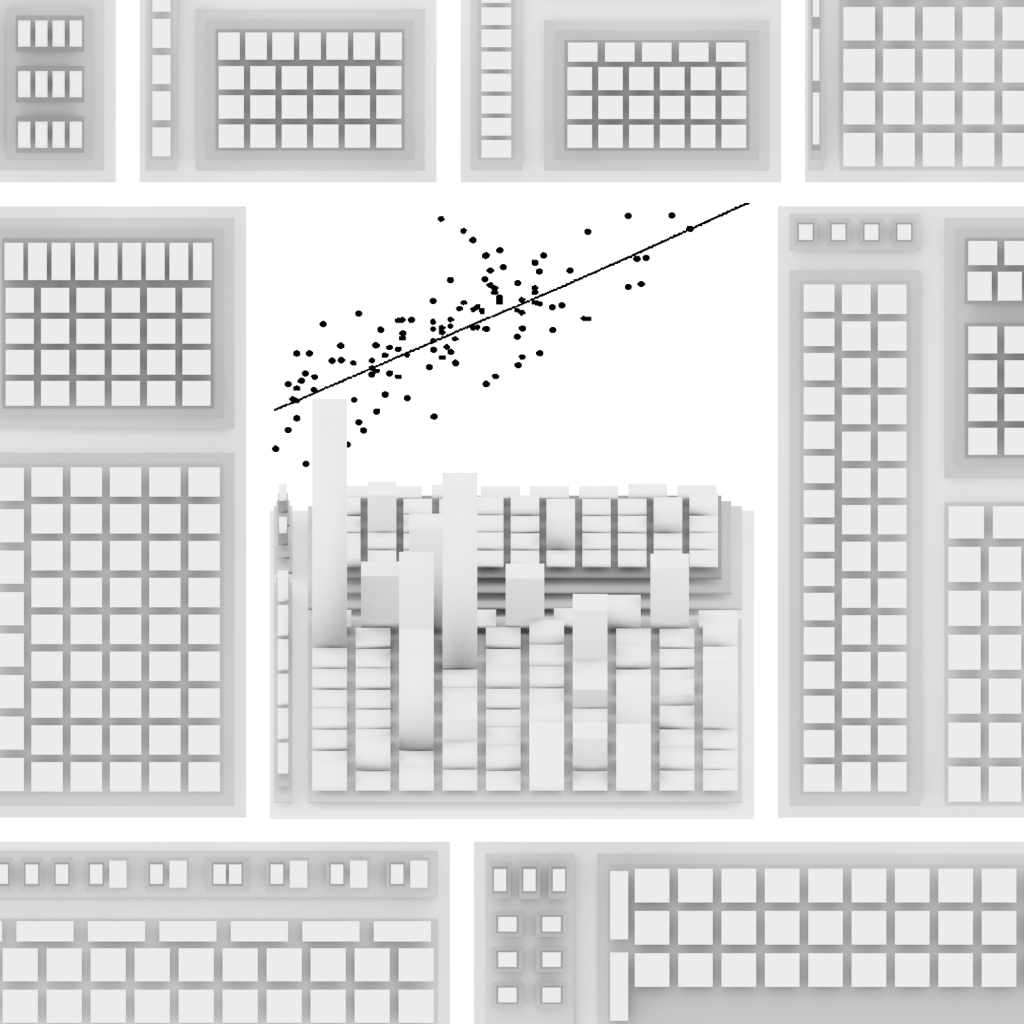
\includegraphics[height=1.1in]{images/future-ortho-scatter}

        \smallskip
        Available Screen Space

        \end{column}

    \end{columns}

\end{frame}

\begin{frame}{Conclusion and Contact Information}

   \begin{columns}

       \begin{column}{0.5\textwidth}

            This talk presented
           \begin{itemize}
                \item a \blueify{node-local tilt transformation} and
                \item \blueify{interactive tilt control}
           \end{itemize}
           in order to facilitate \blueify{exploration of unknown data} using 2D and 2.5D treemaps.

            \bigskip
            Author email addresses:
            \begin{itemize}
                \item \blueify{\underline{daniel.limberger@hpi.de}}
                \item \blueify{willy.scheibel@hpi.de}
                \item \blueify{matthias.trapp@hpi.de}
                \item \blueify{juergen-doellner@hpi.de}
            \end{itemize}

        \end{column}

        \begin{column}{0.42\textwidth}

            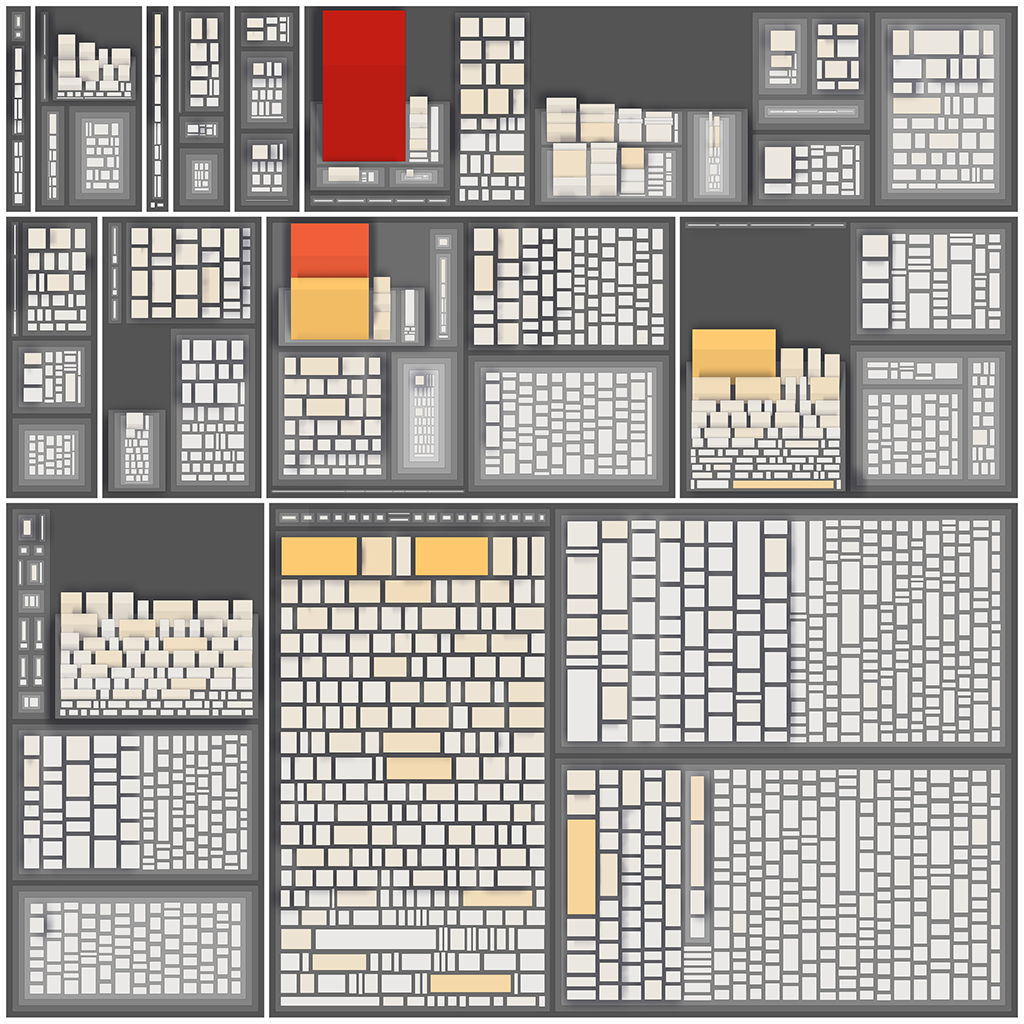
\includegraphics[width=\textwidth]{images/mixed-poco-2-small}

        \end{column}

    \end{columns}

\end{frame}

\begin{frame}[allowframebreaks]{Bibliography}
    \bibliographystyle{acm}
    \setbeamertemplate{bibliography item}{\insertbiblabel}
    \bibliography{references}
    \vfill
\end{frame}

\begin{frame}{Software Maps | Map Theme}

    \begin{columns}

        \begin{column}{0.6\textwidth}
            \Large For a given task, a \blueify{map theme} specifies the\\mapping of attributes to visual variables.
        \end{column}

        \begin{column}{0.34\textwidth}
            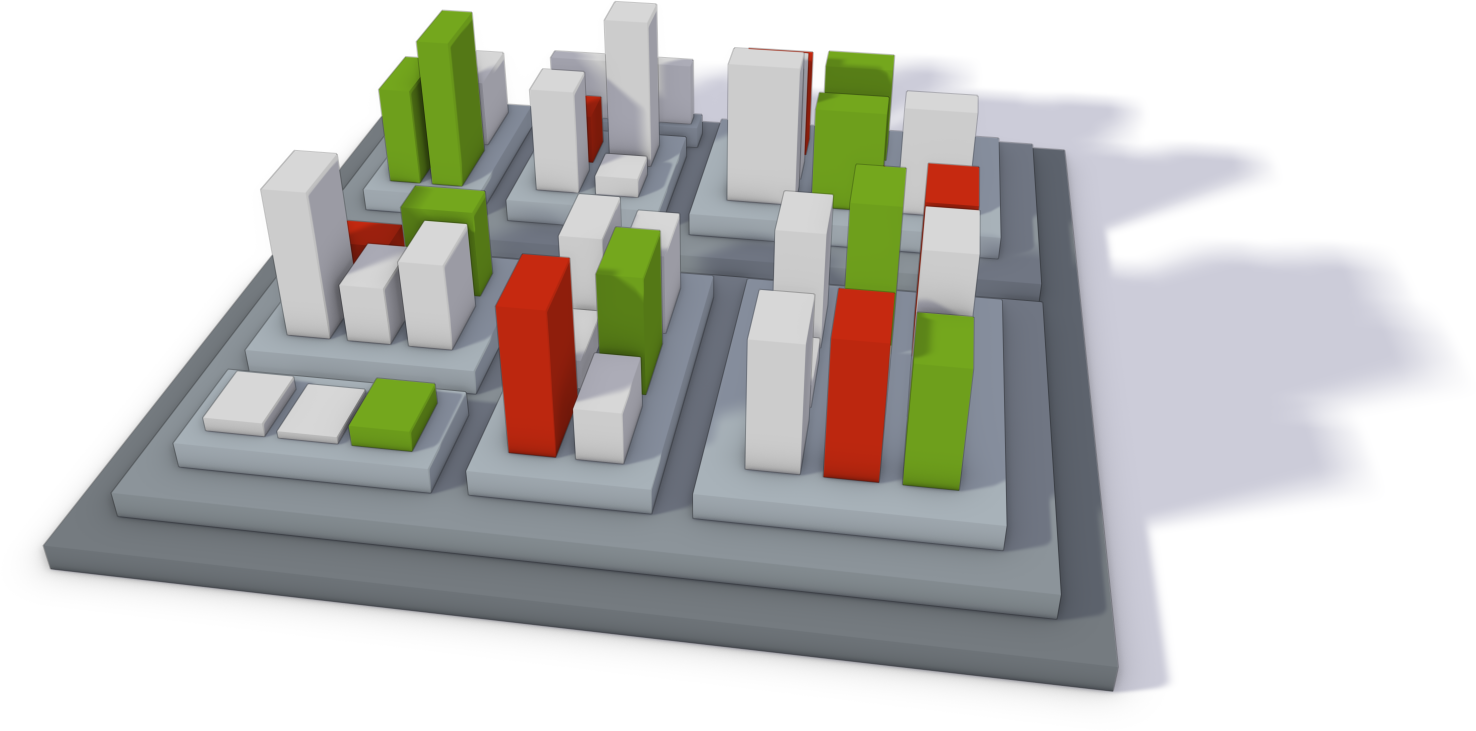
\includegraphics[width=2in]{images/app-maps}
        \end{column}

    \end{columns}

    \medskip
    \normalsize

    \begin{description}

        \pause
        \item[\blueify{Technical Depth}] maps logic lines-of-code to weight, a nesting-level metric to color, and McCabe complexity \cite{McCabe1976}.
        It is used to reveal and monitor the 'technical debts' inherent to a software system's implementation.

        \pause
        \item[\blueify{Risk of Knowledge Drain}] maps logic lines-of-code to weight, the number of active developers to color, and a composite, nesting-level or McCabe based complexity measure indicating difficult-to-comprehend code to height. It is used to identify complex code units known only by few developers and reveal knowledge distribution.

    \end{description}

\end{frame}

\begin{frame}[t]{Software Maps | Goals}

    \bigskip

    \begin{columns}

        \begin{column}{0.65\textwidth}

            Make code quality of software systems visible to \enquote{stakeholders in the development process, particularly, to the management} \cite{Bohnet2011} by means of depicting, e.g., metrics and activity data.

            \bigskip
            \blueify{Depending on the applied map theme Software Maps facilitate}
            \begin{itemize}
                \item exploring structures,
                \item monitoring development processes,
                \item monitoring software quality, and
                \item identifying areas that require attention in the ongoing development process.
            \end{itemize}

        \end{column}

        \begin{column}{0.28\textwidth}
            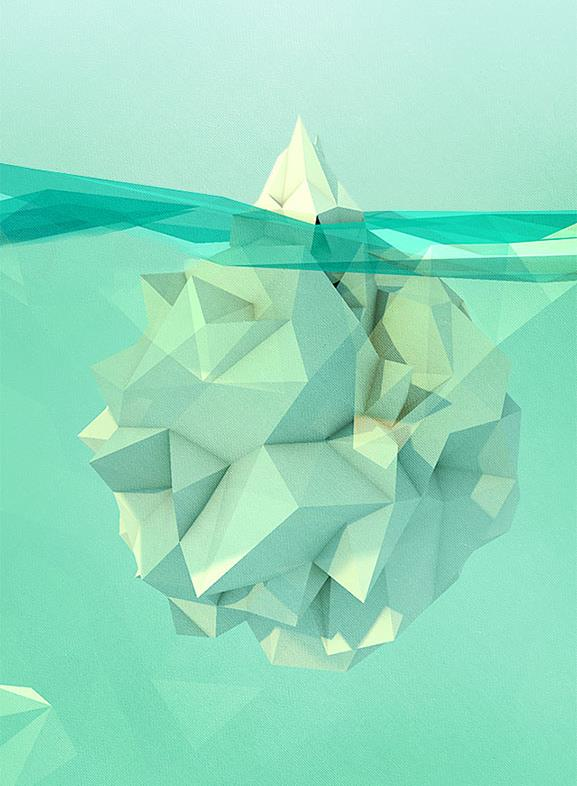
\includegraphics[width=1.5in]{images/iceberg}
        \end{column}

    \end{columns}

\end{frame}

\end{document}

